\documentclass[conference]{IEEEtran}
\IEEEoverridecommandlockouts

\usepackage{cite}
\usepackage{amsmath,amssymb,amsfonts}
\usepackage{graphicx}
\usepackage{textcomp}
\usepackage{xcolor}
\usepackage{booktabs}
\usepackage{siunitx}
\usepackage{url}
\usepackage{hyperref}
\hypersetup{colorlinks=true,linkcolor=blue,citecolor=blue,urlcolor=blue}

\def\BibTeX{{\rm B\kern-.05em{\sc i\kern-.025em b}\kern-.08em
    T\kern-.1667em\lower.7ex\hbox{E}\kern-.125emX}}

\begin{document}

\title{An Open-Source PCB Test Vehicle for Electrical Characterization of Solder-Bonded Micro-LEDs:\\Design, Schematic, and Measurement Workflow\\
{\normalsize Course report — ET4277 + ET4391 — Part 1}}

\author{\IEEEauthorblockN{Daniel Tyukov}
\IEEEauthorblockA{\textit{Department of Microelectronics, ECTM + ITEC}\\
\textit{Delft University of Technology}\\
Delft, the Netherlands \\
Student no. 5714699 \;\textbar\; \texttt{daniel.tyukov@alphait.us}}
}

\maketitle

\begin{figure}[!t]
  \centering
  
\includegraphics[width=0.3\columnwidth]{figures/tudelft_logo.pdf}
\end{figure}

\begin{abstract}
We designed a 93~mm $\times$ 93~mm two-layer FR-4 PCB to characterize how
different solder pastes perform when bonding micro-LEDs. The board carries
26 Würth WL-SFCC 0404 RGB LEDs (8 addressable, 18 in two daisy chains), four
0402 NTCs for forward-voltage thermometry, a 100~$\Omega$ 0.1\% reference
resistor with OPEN/SHORT/LOAD pads for impedance spectroscopy, and a set of
TLM ladders and van der Pauw cloverleaves on the same substrate. Putting all
of this on one PCB means a single cleanroom session yields bond resistance,
contact resistivity, sheet resistance, and junction-to-substrate thermal
resistance from the same hardware. No separate test coupons, no inter-board
correlation. Two 32-pin headers break every active net out to a breadboard.
The board is fab-ready for the Aisler standard pool with ENIG plating; LEDs
are deliberately left unassembled, since the bond joint itself is the
research subject and has to form under controlled cleanroom conditions. What
follows is a walkthrough of the schematic, the characterization methods, the
tools needed to run them, and the four-paste comparison the design was built
for.
\end{abstract}

\begin{IEEEkeywords}
micro-LED, die bonding, solder paste, V$_F$-TSP, electrochemical impedance
spectroscopy, transmission line method, van der Pauw, daisy chain, electrical
characterization, PCB test vehicle
\end{IEEEkeywords}

\section{Introduction}

Mounting a sub-millimeter LED die on a PCB sounds simple until you measure
it. The joint has to carry current with a low voltage drop, pull heat out
of the die fast enough to keep it from cooking itself, and survive whatever
thermomechanical cycling the application throws at it. With SAC305 reflow
paste, the cheap default, the quality of that joint depends on paste
rheology, stencil aperture, reflow profile, and substrate finish
\cite{ji2023polymer,fettke2020lab}. Alternative chemistries (Au-Sn
eutectic \cite{yin2024ausn}, Cu-Cu direct bonding \cite{wang2023cucu},
anisotropic solder films \cite{choi2021sitrab}, polymer-reinforced pastes
\cite{ji2023polymer}) trade one of those parameters for another.

This board extends the v1 design Abdelwahab et al.\ shipped at ECTC 2025
\cite{abdelwahab2025ectc}. The v1 measured bond yield and V$_F$ only. v2
adds three more characterization methods (TLM contact resistivity, van der
Pauw sheet resistance, EIS impedance) on the same substrate, so one
cleanroom session produces a complete electrical fingerprint of whatever
paste-and-reflow combination was run. We deliberately target the Aisler
standard pool, not a semiconductor fab, to keep the boards cheap
(\textasciitilde\euro40 each) and reproducible at any university lab.

\section{Board Architecture (v4.0.7)}

\begin{figure*}[!t]
  \centering
  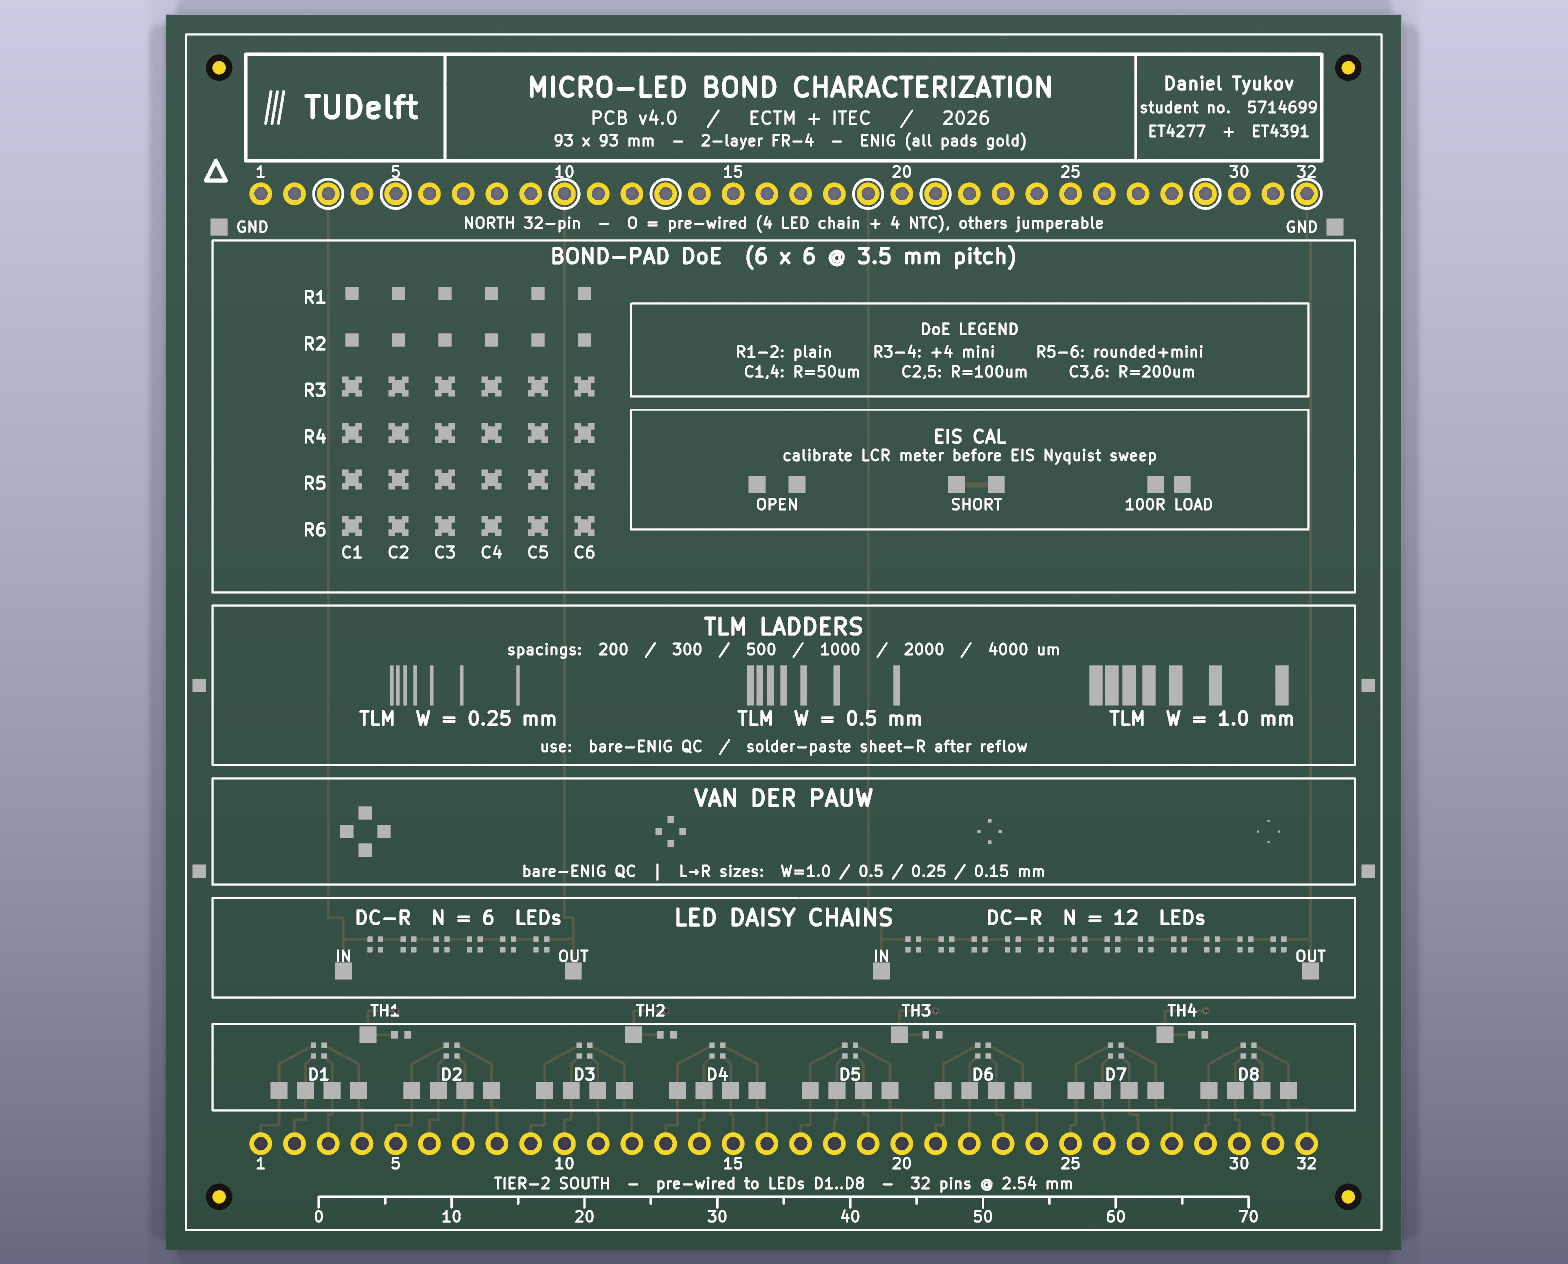
\includegraphics[width=0.42\textwidth]{figures/board_top.png}\hspace{0.04\textwidth}
  
\includegraphics[width=0.42\textwidth]{figures/board_bottom.png}
  \caption{v4.0.7 PCB, 93~mm $\times$ 93~mm, 2-layer FR-4, ENIG finish. Left: top side with
  the four functional zones (title block, DoE bond-pad array + EIS calibration, TLM/VDP test
  structures, LED row + NTCs) and 32-pin north/south breadboard headers.
  Right: bottom side with TUDelft branding, fabrication notes, designer block, and the
  south-header pinout legend that maps the 32 cable wires to the eight LED slots.}
  \label{fig:board}
\end{figure*}

The board (Fig.~\ref{fig:board}) is laid out in five horizontal zones from
top to bottom: (a)~a title block carrying project, designer, and course
metadata; (b)~the 32-pin north header (Würth WR-PHD 61304011121, 1$\times$40
single-row vertical THT cut to 32~pins \cite{wurth_wrphd}), pre-routed to
chain endpoints and NTC sense lines while leaving 24 pins user-jumperable;
(c)~the 6$\times$6 DoE bond-pad array at 3.5~mm pitch with a co-located EIS
calibration block (OPEN/SHORT/LOAD references with the 100~$\Omega$
$\pm$0.1\% Vishay TNPW0603100RBEEA reference resistor \cite{vishay_tnpw});
(d)~three TLM ladders ($W \in \{0.25, 0.5, 1.0\}$~mm, gaps
$\{200, 300, 500, 1000, 2000, 4000\}$~$\mu$m) and four VDP cloverleaves
($W \in \{1.0, 0.5, 0.25, 0.15\}$~mm); (e)~the LED row D1--D8 with the
four Murata NCP15XH103J03RC NTC thermistors \cite{murata_ncp15} interleaved
between LED pairs, two daisy chains (DCL6 with 6 LEDs, DCL12 with 12 LEDs,
both wired through the K$_R$ cathode), and the 32-pin south header that
pre-routes every D1--D8 signal (LED\_VCC + 24 cathodes).

Design rule budget: 0.20~mm minimum copper track and 0.30~mm minimum
copper clearance (both above the Aisler standard-pool 0.15~mm spec by
$\geq$1.3$\times$ and 2$\times$ respectively); 0.30~mm minimum drill;
0.15~mm via annular ring. DRC: 0 violations, 0 unconnected items. ENIG
plating (Ni 4~$\mu$m, Au 0.075~$\mu$m) is mandatory because every probe
pad must be gold for reliable mechanical contact and to receive the
bonded die. Total: 192 footprints --- 69 fab-assembled (4 NTC, 1 resistor,
64 header pins) and 123 customer-handled (26 LED footprints bonded in
cleanroom + 97 bare-ENIG test lands).

\section{Schematic and Net Plan}

The single-sheet A2 schematic in Fig.~\ref{fig:schematic} captures the
36 electrically active components in six functional blocks and 164 named
nets. Bare-pad test structures (TLM, VDP, DoE, probe, TC pads, fiducials,
123 entries) are documented in the design notes block and on the PCB silk
rather than drawn out, since each has no connection beyond its own pad.

\begin{figure*}[!t]
  \centering
  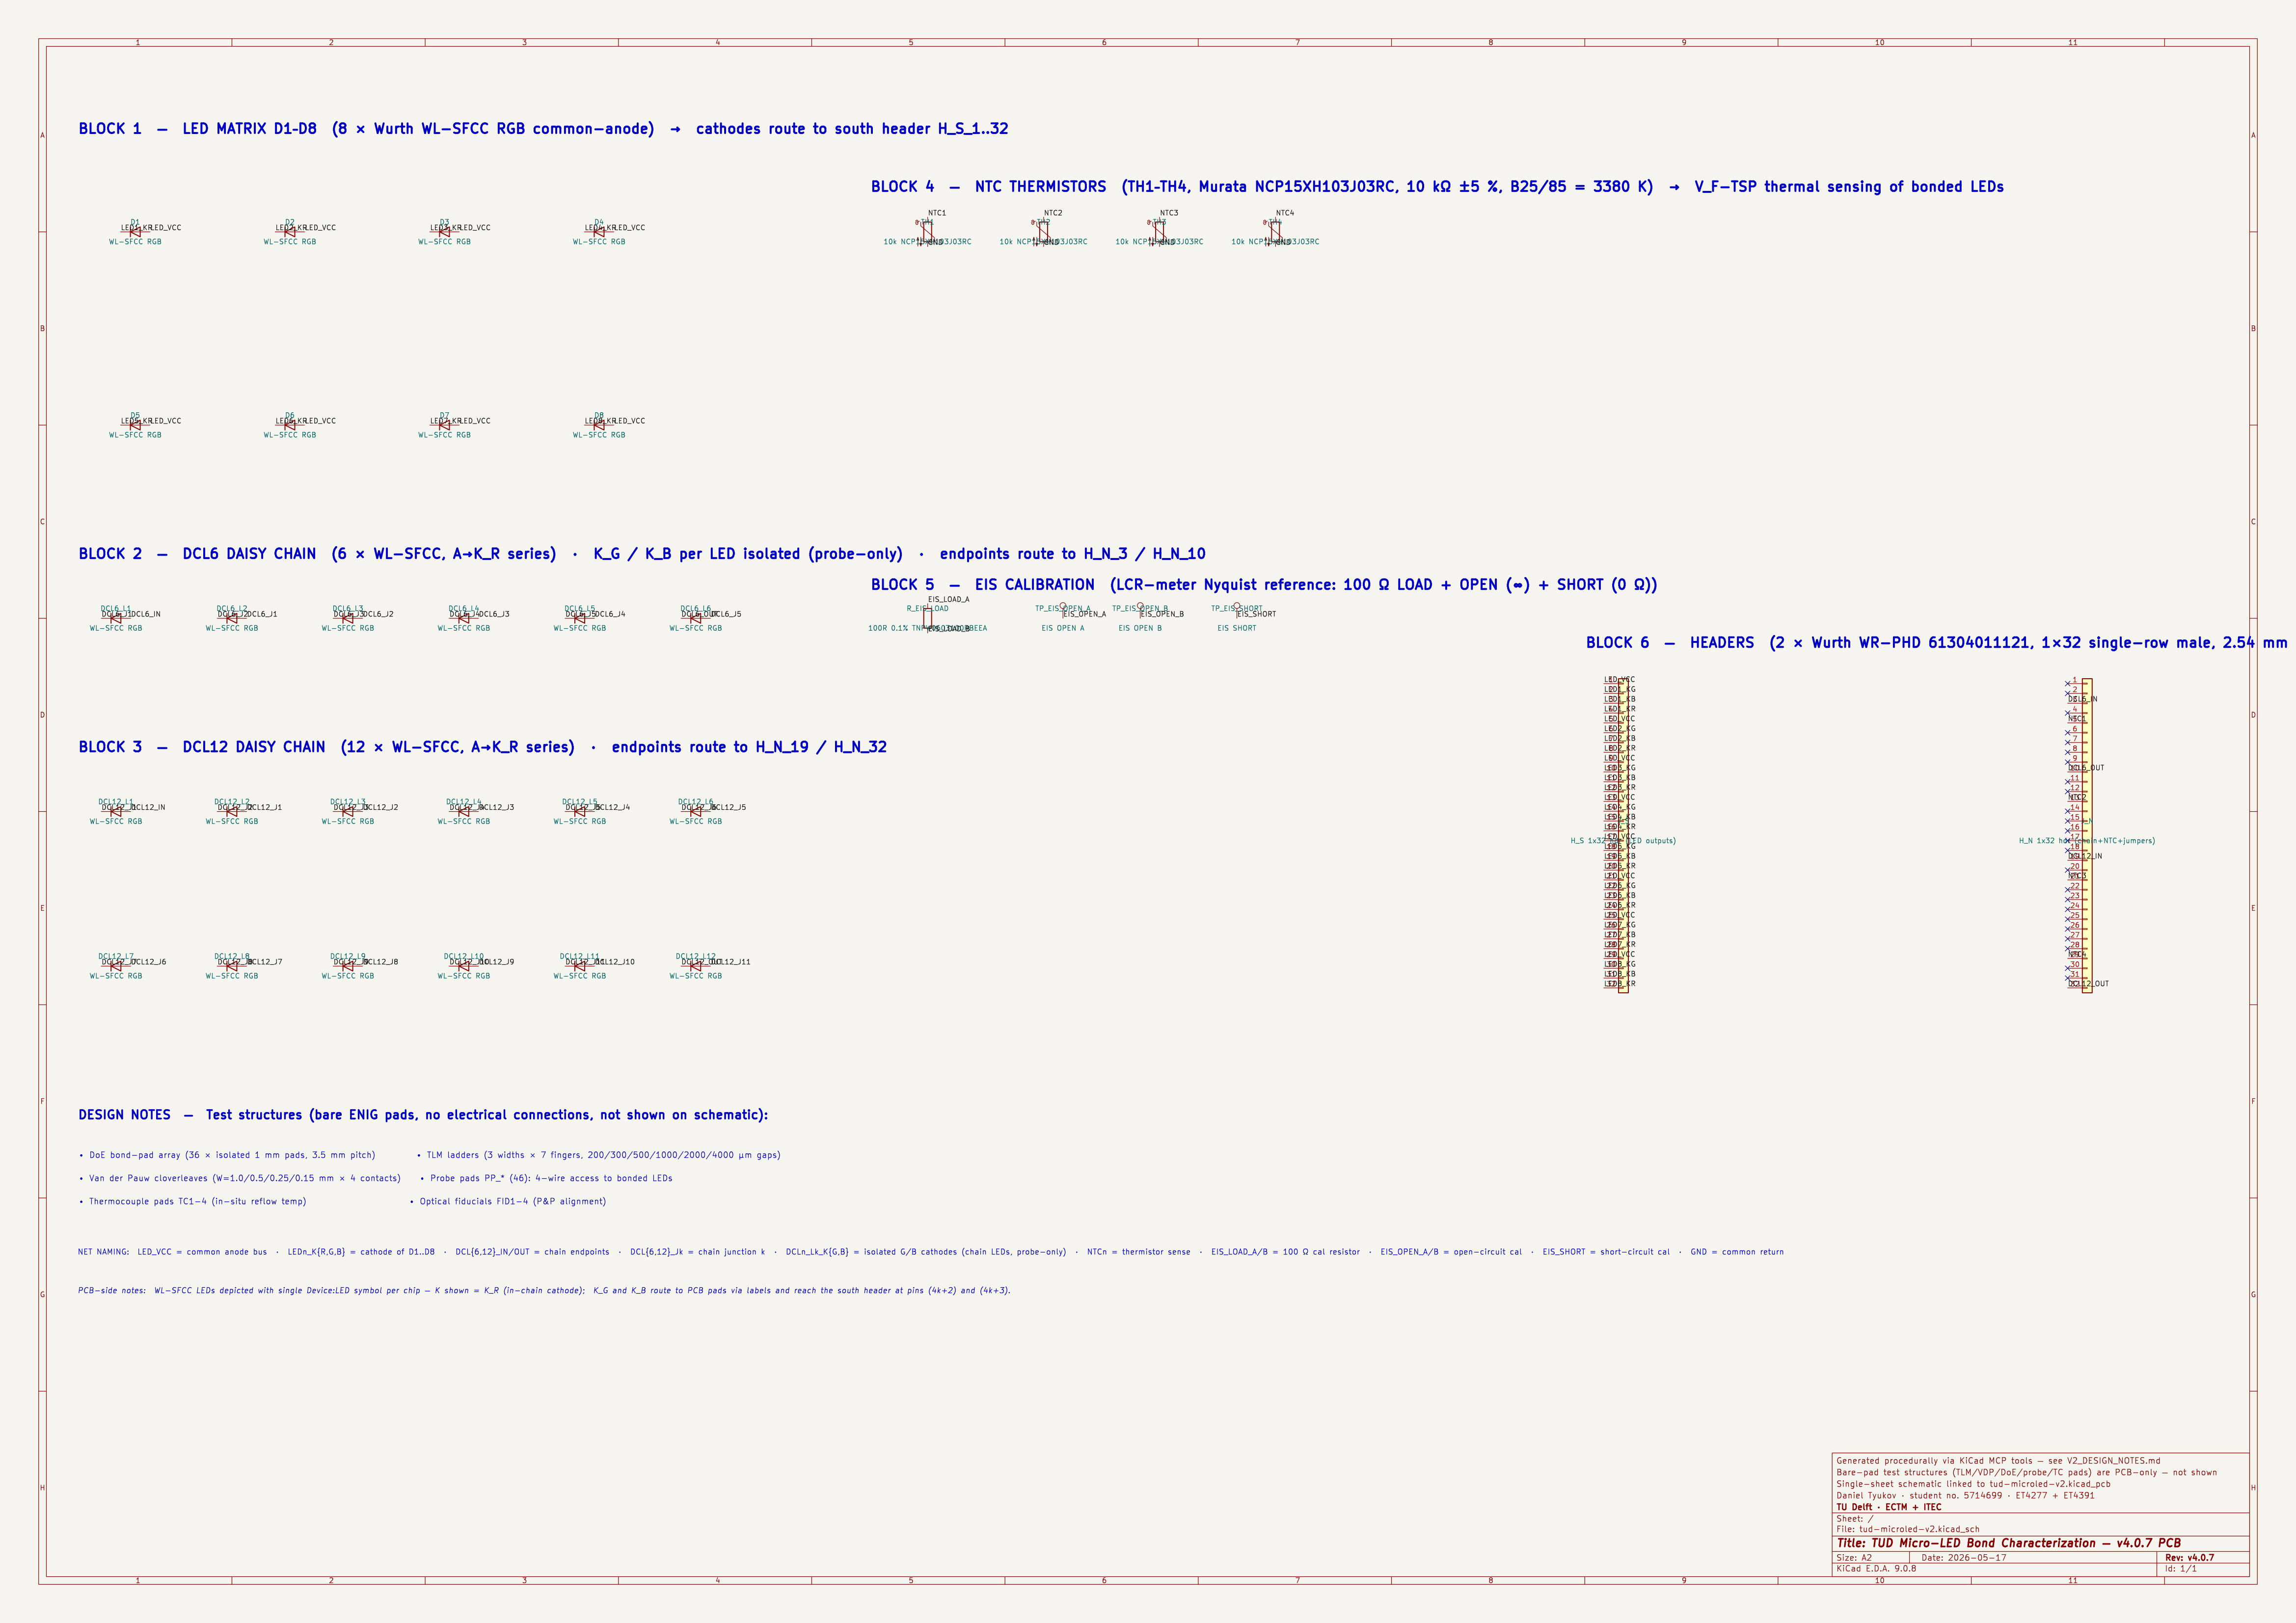
\includegraphics[width=0.97\textwidth]{figures/schematic.png}
  \caption{Single-sheet A2 schematic. Block 1: D1--D8 common-anode LED matrix
  (cathodes routed to south header). Blocks 2--3: DCL6 and DCL12 daisy chains
  (A$\rightarrow$K$_R$ series; K$_G$/K$_B$ per chain LED kept isolated for
  probe-only access). Block 4: TH1--TH4 NTC thermistors for V$_F$-TSP
  thermometry. Block 5: EIS calibration block (LOAD/OPEN/SHORT references).
  Block 6: north + south 32-pin headers with all routed pins labeled and
  no-connect markers on the 24 user-jumperable north pins.}
  \label{fig:schematic}
\end{figure*}

Net naming convention (top-level, for cross-referencing the BOM and PCB):
\texttt{LED\_VCC} is the 8-anode common bus (B.Cu copper pour);
\texttt{LED}$n$\texttt{\_K\{R,G,B\}} are the individual D$n$ cathode signals;
\texttt{DCL\{6,12\}\_IN}/\texttt{OUT} are chain endpoints; \texttt{DCL\{6,12\}\_J}$k$
are internal junctions; \texttt{DCL}$n$\texttt{\_L}$k$\texttt{\_K\{G,B\}} are
the per-chain-LED isolated green/blue cathodes; \texttt{NTC}$n$ are the
four thermistor sense lines; \texttt{EIS\_\{LOAD,OPEN,SHORT\}\_\{A,B\}}
are the calibration probe pads; \texttt{GND} is the common return on the
B.Cu pour.

\section{Electrical Characterization Methods}

Four orthogonal methods exercise the board:

\subsection{Forward-voltage thermometry (V$_F$-TSP)}

A diode's forward voltage at a fixed low current decreases monotonically with
junction temperature; the slope (Temperature Sensing Parameter)
$S \equiv -\partial V_F / \partial T_J$ is approximately constant for any given
device and bias current and is the basis of the standard JEDEC JESD51-1
junction-temperature measurement \cite{roscamabbing2011led,dellacorte2020vftsp}.
For an LED biased at a sense current $I_S \ll I_{op}$,
\begin{equation}
  T_J(t) \;=\; T_{J,0} \;-\; \frac{1}{S}\bigl[V_F(t) - V_{F,0}\bigr],
  \label{eq:vftsp}
\end{equation}
where $V_{F,0}$ is the forward voltage at the calibration temperature $T_{J,0}$.

The four NTCs (TH1--TH4, Murata NCP15XH103J03RC, $R_{25}=10$~k$\Omega$, $B_{25/85}=3380$~K)
sit between the LED pairs and provide the substrate-side reference; we read
the LED V$_F$ across the four bonded contacts via the south header and the
NTC resistance via the north header. The NTC resistance maps to temperature
through the Steinhart-B equation,
\begin{equation}
  \frac{1}{T} \;=\; \frac{1}{T_0} \;+\; \frac{1}{B}\,\ln\!\left(\frac{R}{R_0}\right),
  \label{eq:ntc}
\end{equation}
with $T_0 = 298.15$~K, $R_0 = 10$~k$\Omega$, $B = 3380$~K \cite{murata_ncp15}.
The pulsed sensing protocol of Pangallo et al.\ \cite{pangallo2018direct}
avoids self-heating bias; we use $I_S = 100$~$\mu$A pulses of 1~ms with $10\%$
duty.

The bond-joint thermal resistance is extracted from the transient
$Z_{th}(t)$ response after a step in operating current, deconvolved per
Schwan et al.\ \cite{schwan2024thermal} or via the network-identification
method of Liu et al.\ \cite{liu2019rectangular}. The relevant figure of
merit is the steady-state bond resistance
\begin{equation}
  R_{th,bond} \;=\; \lim_{t \to \infty}\frac{T_J(t) - T_{NTC}(t)}{P_{op}},
\end{equation}
with $P_{op}$ the dissipated electrical power.

\subsection{Electrochemical impedance spectroscopy (EIS)}

EIS sweeps a small AC voltage (typically 10~mV) over $10^{-1}$\,Hz to $10^{6}$\,Hz
and records the complex impedance $Z(j\omega) = Z' + jZ''$. The Nyquist plot
$Z''(Z')$ separates the bond-joint resistance (high-frequency intercept,
$Z' \rightarrow R_s$ as $\omega \rightarrow \infty$) from the diode's
parallel RC dynamics (low-frequency semicircle). For an ideal LED equivalent
circuit (series bond resistance $R_s$, parallel diffusion resistance
$R_p$ with junction capacitance $C_j$),
\begin{equation}
  Z(j\omega) \;=\; R_s \;+\; \frac{R_p}{1 + j\omega R_p C_j}.
  \label{eq:eis}
\end{equation}

Meaningful EIS requires instrument calibration. The board carries three
on-PCB references that the user shorts the LCR/EIS analyzer to before each
sweep: \texttt{EIS\_OPEN} (two isolated 1.27-mm gold pads, $Z\rightarrow\infty$),
\texttt{EIS\_SHORT} (paired pads joined by a solder bridge, $Z \rightarrow 0$),
and \texttt{EIS\_LOAD} (the 100~$\Omega$ $\pm$0.1\% Vishay TNPW0603100RBEEA
thin-film resistor with 25~ppm/K TCR \cite{vishay_tnpw}). The 1.27-mm
square pads are oversized relative to IPC-7351 0603 nominal so they double
as four-wire Kelvin probe lands.

\subsection{Transmission Line Model (TLM)}

TLM extracts the sheet resistance $R_{sh}$ of the metallization and the
specific contact resistivity $\rho_c$ between the bond pad and the LED
electrode from the resistance measured between successive finger pairs at
known gaps $d$ \cite{wang2023cucu,yin2024ausn}. For $N$ identical
contacts of width $W$ and characteristic length $L_T$,
\begin{equation}
  R_{tot}(d) \;=\; \frac{R_{sh}}{W}\,d \;+\; 2\,R_c,
  \quad
  R_c \;=\; \frac{R_{sh}\,L_T}{W}\coth\!\left(\frac{L}{L_T}\right),
  \label{eq:tlm}
\end{equation}
where $R_c$ is the contact resistance and $L$ the contact length. A
linear fit of $R_{tot}$ vs $d$ yields $R_{sh}$ from the slope and $2R_c$
from the intercept; $\rho_c$ then follows from
$\rho_c = R_c \cdot W \cdot L_T \cdot \tanh(L/L_T)$.

Our three ladders span $W \in \{0.25, 0.5, 1.0\}$~mm (so the contact-width
dependence of the transfer length can also be tested) and gaps
$\{200, 300, 500, 1000, 2000, 4000\}$~$\mu$m. The smallest gap (200~$\mu$m)
is above the Aisler standard-pool fabrication minimum, so all ladders are
manufacturable in the same run as the LED-side traces and the measurement
references the same ENIG surface that the bond contacts see.

\subsection{Van der Pauw (VDP) sheet resistance}

VDP four-point measurement on a symmetric cloverleaf gives a direct
absolute $R_{sh}$ value, independent of contact geometry, from the
implicit relation
\begin{equation}
  \exp\!\left(-\pi\,\frac{R_A}{R_{sh}}\right) \;+\;
  \exp\!\left(-\pi\,\frac{R_B}{R_{sh}}\right) \;=\; 1,
  \label{eq:vdp}
\end{equation}
with $R_A$ and $R_B$ the two transverse four-point resistances measured at
$90^\circ$ rotation around the sample \cite{wang2023cucu}. For a
symmetric clover ($R_A \approx R_B \equiv R$),
$R_{sh} = (\pi/\ln 2)\,R$. Our four cloverleaves
($W \in \{1.0, 0.5, 0.25, 0.15\}$~mm) cross-check the TLM
slope and quantify width-dependent edge effects.

\subsection{Daisy-chain bond-yield QC}

The DCL6 and DCL12 chains place 6 (resp.\ 12) WL-SFCC LEDs in series via
their K$_R$ cathode, exercising $2N$ bonds per chain (anode + K$_R$ cathode
on each die). A current-voltage sweep across the chain endpoints
(\texttt{DCL$n$\_IN}/\texttt{OUT} on the north header) detects any open
or high-resistance bond as a discontinuity in $I(V)$ or as a chain
$V_F$ that significantly exceeds the expected $N \cdot V_{F,\text{nominal}}$.
For WL-SFCC red at 10~mA, $V_{F,R} \approx 2.05$~V \cite{wurth_wlsfcc},
so DCL12 yields a clean go/no-go criterion around 24--25~V drive at
10~mA. The K$_G$ and K$_B$ cathodes of each chain LED are routed to
isolated probe pads so the chain pass/fail can be cross-checked
per-die and per-color.

\section{Tooling and Assembly Workflow}

\textbf{Software.} KiCad 9.0.8 for the project (\texttt{tud-microled-v2.kicad\_pro});
the \texttt{.kicad\_pcb} is procedurally generated by
\texttt{tools/generate\_pcb\_text.py} and the schematic by the same KiCad
MCP tool chain that built Figure~\ref{fig:schematic}. Fab outputs are
exported with \texttt{kicad-cli}: gerbers + drill (Aisler reads native
\texttt{.kicad\_pcb} but the bundle is shipped as a fallback), pick-and-place
CSV, top/bottom review PDFs, the 3D STEP model, and the Beagle-format BOM
(\texttt{tools/gen\_aisler\_bom.py}).

\textbf{Fabrication.} The board ships to Aisler (Aachen/Eindhoven) for
the standard-pool 2-layer FR-4 1.55~mm process with ENIG. Beagle assembly
soldering covers the 4 NTCs, the 1 EIS load resistor, and the 64 pin-header
pins (2 strips of 32, cut from 1$\times$40). The 26 WL-SFCC LED footprints
are flagged \emph{do not populate} (DNP) in the BOM and assembly notes,
because they are the research subject and are bonded by the customer
in the TU~Delft cleanroom under controlled paste / reflow-profile /
die-bonder conditions. Expected cost: \textasciitilde\euro115--125 for
three fully assembled boards delivered.

\textbf{Bonding.} LED placement uses the Tresky T-3000-PRO die bonder
(envelope 95~mm $\times$ 95~mm, our 93~mm board fits with 1~mm margin).
Solder paste is stencilled through a 100~$\mu$m laser-cut stencil keyed
to the WL-SFCC pad layout (4 corner pads, 0.4~mm $\times$ 0.4~mm at
0.8~mm pitch per the Würth recommendation \cite{wurth_wlsfcc}). Reflow
follows IPC J-STD-020E with peak temperature 245--260~$^{\circ}$C per the
solder paste vendor.

\textbf{Measurement.} Lab equipment used in our cleanroom: Keithley 2450
SourceMeter for V$_F$-TSP and I-V sweeps; Solartron 1260A FRA + 1296A
dielectric interface for EIS; HP4156 parameter analyzer for TLM/VDP;
Tresky as bonder; T-type thermocouples soldered to the four \texttt{TC$n$}
gold pads for in-situ reflow temperature logging. Probe access is via
1.27~mm Kelvin probes on the \texttt{PP\_*} pads or via ribbon-cable
breakouts from the 32-pin headers.

\section{Solder-Mixture Experiment Plan}

The board's primary research target is to compare commercial solder pastes
of different chemistries on identical LED-and-substrate hardware. We
nominate four candidates that span the relevant trade space:
\begin{enumerate}
  \item \textbf{SAC305} (Sn 96.5\% / Ag 3.0\% / Cu 0.5\%) — industry
        baseline.
  \item \textbf{SAC0307} (low-silver variant) — lower cost, slightly
        worse thermal cycling, similar V$_F$ drop.
  \item \textbf{Au-Sn 80/20 eutectic} — high-temperature reference
        \cite{yin2024ausn} with documented best-in-class contact resistivity.
  \item \textbf{Polymer-reinforced SAC305} — emerging impact-resistant
        chemistry \cite{ji2023polymer} relevant to flexible-display
        applications.
\end{enumerate}

For each paste we run a 3-board batch (one trial + one real + one spare,
matching Aisler's bundling). On each board we measure: chain-yield ($N_{ok}/N$
across DCL6 and DCL12), per-LED V$_F$ at 10~mA, R$_{th,bond}$ from
V$_F$-TSP transient, $R_s$ + $R_p$ + $C_j$ from EIS fit to
\eqref{eq:eis}, and $\rho_c$ from TLM fit to \eqref{eq:tlm}.
Cross-board variance gives statistical bounds on each paste's process
window.

Beyond the solder-mixture comparison the board also supports
investigations that re-use the same characterization plumbing: capillary
self-alignment yield as a function of pad geometry (the DoE 6$\times$6
array with its plain / minis / rounded variants), reflow profile
optimization (T$_C$ vs T$_{C-5}$ tracking on the TC pads), and bond
ageing studies (the chains can be loaded with a programmable
current source to drive thermomechanical fatigue).

\section{Conclusion}

We have presented a self-contained 93~mm $\times$ 93~mm PCB test vehicle
that consolidates four electrical-characterization methods
(V$_F$-TSP thermometry, EIS, TLM, VDP) plus daisy-chain yield QC on a
single substrate, enabling a complete bond-quality fingerprint from
one cleanroom session. The board is fab-ready on the Aisler standard
pool with ENIG plating, with a 0-DRC-violation budget and conservative
2$\times$ margin over the published manufacturing minima. The
accompanying schematic, BOM, and tooling pipeline make the design
reproducible. Part~2 of this report will present the first
electrical-characterization results from the four-paste comparison
once the boards arrive and the cleanroom bonding session is complete.

\section*{Acknowledgment}

This work extends the v1 board of A.\ Abdelwahab et al.\
\cite{abdelwahab2025ectc} and benefits from supervision by
M.\ Mastrangeli and H.\ van Zeijl (TU~Delft ECTM). Industrial
collaboration with R.\ van Hoorn and H.\ Kuipers (ITEC~B.V./Nexperia)
provided the bonding-process context. Financed by ITEC~B.V.\
and co-financed by the Netherlands Enterprise Agency (RVO).

\bibliographystyle{IEEEtran}
\bibliography{refs}

\end{document}
